\title{Study Guide for Midterm 1}
\author{Dr. Jordan Hanson - Whittier College Dept. of Physics and Astronomy}
\date{\today}
\documentclass[10pt]{article}
\usepackage[a4paper, total={18cm, 27cm}]{geometry}
\usepackage{outlines}
\usepackage{graphicx}
\begin{document}
\maketitle

\section{Chapter 1 - Introductory Concepts}
\begin{figure}[ht]
\centering
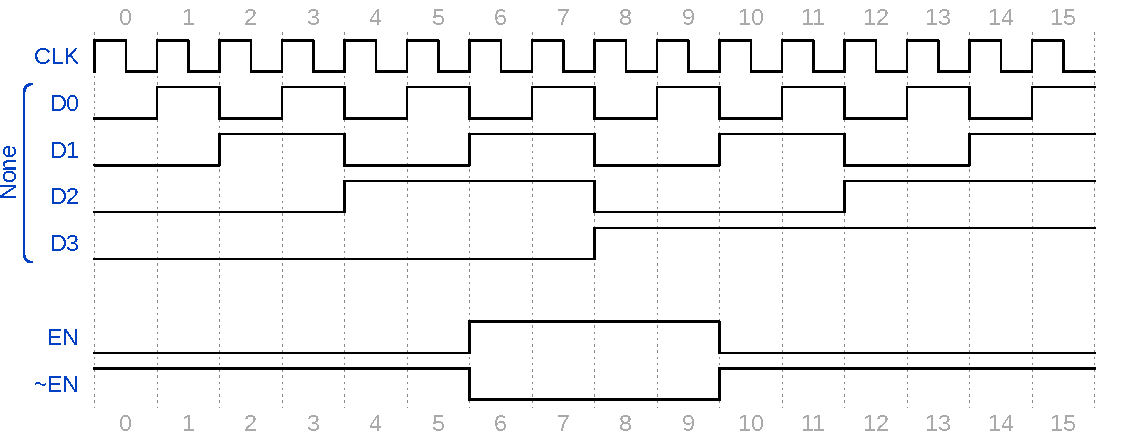
\includegraphics[width=0.6\textwidth]{timingExample6.pdf}
\caption{\label{fig:timing1} A timing diagram including a clock signal (CLK), a 4-bit parallel data stream (D0-D3), and enable/disable signals (EN/$\sim$EN).}
\end{figure}
\begin{enumerate}
\item Consider Fig. \ref{fig:timing1}. (a) What is the duty cycle of each $D_{\rm i}$ signal? (b) Consider the bitstreams of $D_{\rm i}$.  What does the sequence of numbers represent? \\ \vspace{1.0cm}
\item (a) Imagine that $D_i$ signals enter a NAND gate, along with the $\sim$EN signal.  Draw the resulting timing diagram. \\ \vspace{1.5cm}
\item Suppose $D_i$ represents parallel data with a clock frequency of 4 MHz.  (a) What is the total bitrate (bits per second)?  (b) What would be the bit rate if the system was serial instead of parallel? \\ \vspace{1cm}
\end{enumerate}

\section{Chapter 2 - Number Systems, Operations, and Codes}

\begin{enumerate}
\item Convert to binary: (a) 1024 (decimal) (b) 0xBBBB (hex) (c) -2048 (decimal) \\ \vspace{1.5cm}
\item Convert to hex: (a) 65535 (decimal) (b) 1000100010001000 (binary) \\ \vspace{1cm}
\item Convert to \textit{octal}, in which \textbf{the base is 8}: 1024 (decimal). \\ \vspace{1cm}
\item Consider the gray code angular encoder in Fig. \ref{fig:grayCode}.  (a) If the shaft rotates 180 degrees, how many bit changes occur?  (b) If it rotates 180 degrees, and the initial gray code is 0000, what is the final gray code?  (c) With 4-bit gray code, how many distinct angles can the shaft encode?  What is 360 degrees divided by this number (i.e. the angular precision)? (d) What would be the angular precision of an 8 bit encoder? \\ \vspace{2cm}
\end{enumerate}
\begin{figure}[hb]
\centering
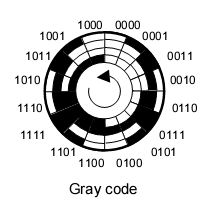
\includegraphics[width=0.2\textwidth]{grayCode1.png}
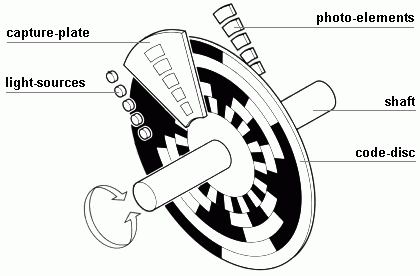
\includegraphics[width=0.3\textwidth]{grayCode2.png}
\caption{\label{fig:grayCode} A gray code shaft encoder, or angular encoder, reports the angular position of an object digitally, using the gray code.}
\end{figure}

\section{Chapter 3 - Logic Gates}
\begin{figure}[ht]
\centering
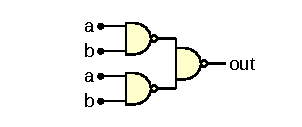
\includegraphics[width=0.3\textwidth]{gateExample1.pdf}
\caption{\label{fig:gates1} Examples of logic gate combinations.}
\end{figure}
\begin{enumerate}
\item Generate the truth tables for the gate diagrams in Fig. \ref{fig:gates1}. Pay attention to the domain.  \\ \vspace{3cm}
\item Identify the actions of the gate combinations in the previous problem from the truth tables.  (a) Fig. \ref{fig:gates1}, left:\rule{3cm}{0.1mm} (b) Fig. \ref{fig:gates1}, middle:\rule{3cm}{0.1mm} (c) Fig. \ref{fig:gates1}, right:\rule{3cm}{0.1mm}.
\item Suppose the signals in Fig. \ref{fig:timing2} are fed into the circuit in Fig. \ref{fig:gates1}, right.  Fill in the S and Cout signals in Fig. \ref{fig:timing2}.
\item Imagine a system for an electronic door lock which requires two electronic keys (two signals), S1 and S2.  The circuit has a red LED, a yellow LED, and a green LED.  The system unlocks when the output LOCK signal is LOW, caused by a LOW S1 and a LOW S2.  The red LED is activated when S1 and S2 are both HIGH.  The yellow LED is activated when S1 and S2 are different.  The green LED is activated when the system is unlocked.  \textit{By default, S1 and S2 are HIGH.} Draw the solution below.  \\ \vspace{4cm}
\end{enumerate}
\begin{figure}[hb]
\centering
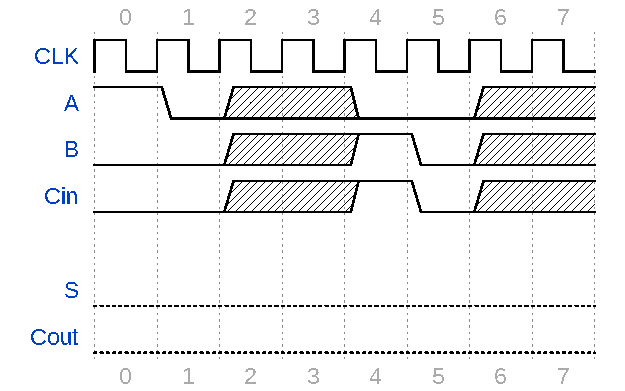
\includegraphics[width=0.5\textwidth]{timingExample2.pdf}
\caption{\label{fig:timing2} An example timing diagram for Fig. \ref{fig:gates1}, right.  The shaded regions indicate ``don't care'' conditions, or times when the data is not relevant.}
\end{figure}

\section{Chapter 4 - Boolean Algebra and Logic Simplification}
\begin{figure}[ht]
\centering
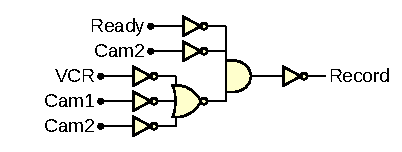
\includegraphics[width=0.4\textwidth]{gateExample4.pdf}
\caption{\label{fig:gates2} A gate combination triggering a signal named ``record.''}
\end{figure}
\begin{enumerate}
\item Consider the circuit in Fig. \ref{fig:gates2}.  (a) Write a logic expression for \textit{Record}. (b) Simplify the expression to as minimal a form as possible. (c) Are any signals or gates unnecessary? \\ \vspace{3cm}
\item Consider again the logic expression that represents the circuit in Fig. \ref{fig:gates2}. (a) Write the corresponding domain-4 Karnaugh map.  (b) Use the Karnaugh map to produce the S-POS expression and truth table. \\ \vspace{3cm}
\end{enumerate}

\section{Chapter 5 - Combinatorial Logic Analysis}
\label{sec:comb}
\begin{figure}[ht]
\centering
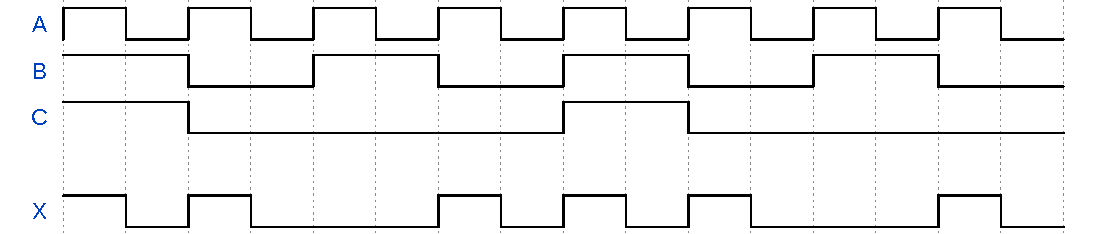
\includegraphics[width=0.5\textwidth]{timingExample3.pdf}
\caption{\label{fig:timing3} Timing diagram for Sec. \ref{sec:comb}.}
\end{figure}
\begin{enumerate}
\item (a) Draw the circuit corresponding to the timing diagram in Fig. \ref{fig:timing3}.  (b) Create the Karnaugh map.  (c) Using the Karnaugh map, write the simplest expression for this logic function and re-draw the circuit.
\end{enumerate}

\end{document}